\label{chap:pt1_state_of_the_art}

The problem of determining a fixture layout that maximizes workpiece stability has been widely studied in the literature. One class of approaches formulates fixture layout as a mathematical optimization problem, often coupled with Finite Element Analysis (FEA)~\cite{bhavikatti2005finite} to evaluate workpiece deformation. Menassa and DeVries~\cite{menassa1991optimization} proposed the use of the Broyden--Fletcher--Goldfarb--Shanno (BFGS) optimization algorithm to determine fixture support locations that minimize deformation. This direction was further explored by Cai et al.~\cite{cai1996deformable}, who combined nonlinear programming with FEA to optimize fixture layouts under a given force, while Camelio et al.~\cite{camelio2004impact} later extended the same approach to minimize shape variations in assembled products. Li and Melkote~\cite{li2001optimal} applied Sequential Quadratic Programming (SQP) to jointly optimize fixture layout and clamping forces. Subsequently, Li et al.~\cite{li2010variation} proposed a flexible fixture system for sheet metal assembly based on assembly variation analysis using the Lagrangian conditional extremum method, while Zhang et al.~\cite{zhang2010fixture} developed a nonlinear optimization model solved using the Augmented Lagrangian method.

Evolutionary and meta-heuristic optimization techniques have also been widely investigated. Kulankara et al.~\cite{kulankara2002iterative} proposed a Genetic Algorithm (GA) for the simultaneous optimization of fixture positions and clamping forces. Shortly afterwards, Y.~Gene Liao~\cite{liao2003genetic} introduced a two-phase GA to identify and refine locating and clamping zones in sheet-metal assembly. Padmanaban et al.~\cite{padmanaban2009machining} combined FEA with discrete and continuous Ant Colony Algorithms (ACA) to reduce sheet metal deformation. Sundararaman et al.~\cite{sundararaman2016optimization} proposed a fixture layout optimization approach combining Response Surface Methodology (RSM), Genetic Algorithms (GA), and Particle Swarm Optimization (PSO), reporting superior performance with PSO. More recently, Liu et al.~\cite{liu2024fixture} introduced an Improved Particle Swarm Optimization (IPSO) algorithm for the fixture layout optimization of large thin-walled parts.

Learning-based methods have recently emerged as an alternative strategy. Selvakumar et al.~\cite{selvakumar2013design} combined Artificial Neural Networks (ANNs) with Design of Experiments (DOE) for machining fixture layout optimization. Wang et al.~\cite{wang2016optimal} integrated neural networks with the Bat Algorithm (BA) to minimize workpiece deformation. Low et al.~\cite{low2020study} proposed a Reinforcement Learning (RL) framework for fixture design, while Wang et al.~\cite{wang2025smartfixture} presented a physics-guided RL approach in which the agent is trained through interaction with an FEA-based simulation.

\begin{figure}[t]
	\centering
	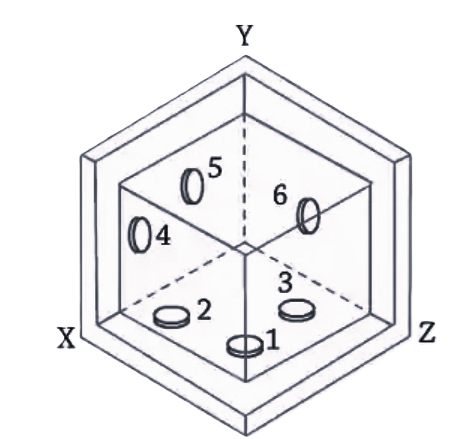
\includegraphics[width=0.35\textwidth]{figures/locating_principle.png}
	\caption{Example of the application of the ``3-2-1'' locating principle for the stabilization of a workpiece}
	\label{fig:locating_principle}
\end{figure}

Although numerous studies on fixture layout optimization exist in the literature, few focus on suction cup fixtures with characteristics similar to those used in wood industry. Most existing research has been conducted in the \emph{metal industry}, where the objective is to determine the number and placement of fixtures according to the ``$N$-2-1'' locating principle in order to minimize workpiece deformation. The ``$N$-2-1'' principle is a generalization of the classical ``3-2-1'' locating scheme. In the latter, three locators constrain the primary datum plane, two constrain the secondary datum, and one constrains the tertiary datum, thereby fully restricting the six rigid-body degrees of freedom of the workpiece, as shown in Figure~\ref{fig:locating_principle}. The ``$N$-2-1'' principle replaces the three primary locators with $N$ locators, while retaining two and one locators on the secondary and tertiary datum planes~\cite{wang2016optimal}.

However, this principle cannot be directly applied to work centers in the wood industry, where the workpiece can only be supported from below. Furthermore, the fixtures adopted in the metal industry generally differ from those used in wood industry, as they typically do not allow rotation. While allowing fixture rotation can significantly improve workpiece stability, it also substantially increases the number of possible solutions and therefore the complexity of the optimization problem.
